\documentclass[12pt, %
openright, 
oneside, %
%twoside, %TCC: Se seu texto tem mais de 100 páginas, descomente esta linha e comente a anterior
a4paper,    %
%english,   %
brazil]{facom-ufu-abntex2}

\usepackage[brazil]{babel}
\usepackage{graphicx}
\graphicspath{{figuras/}{pictures/}{images/}{./}} % where to search for the images

\newcommand{\blue}[1]{\textcolor{blue}{#1}}
\newcommand{\red}[1]{\textcolor{red}{#1}}


\autor{Pedro Henrique Bufulin de Almeida} %TCC
\data{2021}
\orientador{Pedro Frosi Rosa} %TCC
%\coorientador{Algum?} %TCC

% ---
% Informações de dados para CAPA e FOLHA DE ROSTO
% ---

\titulo{Sistema de vigilância \textit{\foreignlanguage{english}{open source}} e customizável} %TCC

\hypersetup{pdfkeywords={palavra 1}{palavra 2}{palavra 4}{palavra 4}{palavra 5}} %TCC

\begin{document}
\frenchspacing

% ----------------------------------------------------------
% ELEMENTOS PRÉ-TEXTUAIS
% ----------------------------------------------------------
%\pretextual
\imprimircapa
\imprimirfolhaderosto

% ---
% Inserir folha de aprovação
% ---
%
% \includepdf{folhadeaprovacao_final.pdf} %TCC: depois de aprovado o trabalho, descomente esta linha e comente o próximo bloco para incluir scan da folha de aprovação.
%
\begin{folhadeaprovacao}

	\begin{center}
		{\ABNTEXchapterfont\large\imprimirautor}

		\vspace*{\fill}\vspace*{\fill}
		{\ABNTEXchapterfont\bfseries\Large\imprimirtitulo}
		\vspace*{\fill}

		\hspace{.45\textwidth}
		\begin{minipage}{.5\textwidth}
			\imprimirpreambulo
		\end{minipage}%
		\vspace*{\fill}
	\end{center}

	Trabalho aprovado. \imprimirlocal, 01 de novembro de 2016: %TCC:

	\assinatura{\textbf{\imprimirorientador} \\ Orientador}
	\assinatura{\textbf{Professor}}% \\ Convidado 1} %TCC:
	\assinatura{\textbf{Professor}}% \\ Convidado 2} %TCC:
	%\assinatura{\textbf{Professor} \\ Convidado 3}
	%\assinatura{\textbf{Professor} \\ Convidado 4}

	\begin{center}
		\vspace*{0.5cm}
		{\large\imprimirlocal}
		\par
		{\large\imprimirdata}
		\vspace*{1cm}
	\end{center}

\end{folhadeaprovacao}
% ---

%%As seções dedicatória, agradecimento e epígrafe não são obrigatórias.
%%Só as mantenha se achar pertinente.

% ---
% Dedicatória
% ---
%\begin{dedicatoria}
%   \vspace*{\fill}
%   \centering
%   \noindent
%   \textit{Dedico a \lipsum[10]}  %TCC:
%   \vspace*{\fill}
%\end{dedicatoria}
% ---

% ---
% Agradecimentos
% ---
%\begin{agradecimentos}
%Agradeço a \lipsum[30]. %TCC:
%\end{agradecimentos}
% ---

% ---
% Epígrafe
% ---
%\begin{epigrafe}
%    \vspace*{\fill}
%	\begin{flushright}
%		\textit{``Alguma citação que ache conveniente? \lipsum[10]''} %TCC:
%	\end{flushright}
%\end{epigrafe}
% ---

\begin{resumo} %TCC:
	Os sistemas de vigilância carecem de soluções
	que sejam customizáveis. Apesar de existirem no mercado câmeras que fazem a gravação e o armazenamento de
	imagem, elas o fazem com com baixa resolução e limitações de espaço de memória severas. Mesmo os equipamentos
	de monitoramento mais sofisticados, como os que possuem reconhecimento de imagem, limitam o usuário de aprimorar
	essas funções por ter o \textit{\foreignlanguage{english}{software}} como \textit{\foreignlanguage{english}{closed source}}.
	Além disso, as soluções providas pela segurança pública ou privada, quando existem, podem usar as imagens
	coletadas para seus próprios benefícios, o que afeta a privacidade do indivíduo. Este trabalho propõe uma solução que seja
	fácil de implementar, com ferramentas prontas para uso e completamente customizável por ser \textit{\foreignlanguage{english}{open source}}.
	Dadas essas características, surge o chamado \textit{\foreignlanguage{english}{Self-Sovereign Camera System}} (SSCS)
	\vspace{\onelineskip}

	\noindent
	\textbf{Palavras-chave}: código  aberto, visão computacional, IP câmera, streaming multimídia.  %TCC:
\end{resumo}

\begin{resumo}[Abstract]

	Surveillance systems lack customizable solutions. Despite the existence of
	cameras on the market that handle both recording and storage of images, they do
	so at low resolution and with severe memory space limitations. Even the most
	sophisticated monitoring equipment, such as those with image recognition
	capabilities, restrict the user from enhancing these features due to the
	software being closed source. Furthermore, solutions provided by public or
	private security, when available, may use the collected images for their own
	benefit, affecting individual privacy. This work proposes a solution that is
	easy to implement, equipped with ready-to-use tools, and fully customizable as
	it is open source. Given these characteristics, the so-called Self-Sovereign
	Camera System (SSCS) emerges.

	\vspace{\onelineskip}
	\noindent
	\textbf{Keywords}: open source, computer vision, IP camera, multimedia streaming.
\end{resumo}

% ---
% inserir lista de ilustrações
% ---
\pdfbookmark[0]{\listfigurename}{lof}
\listoffigures*
\cleardoublepage
% ---

% ---
% inserir lista de tabelas
% ---
\pdfbookmark[0]{\listtablename}{lot}
\listoftables*
\cleardoublepage
% ---

% ---
% inserir lista de abreviaturas e siglas
% ---
\begin{siglas} %TCC: 

	\item[SSCS] Self-Sovereign Camera System
	\item[CAGR] Compound annual growth rate, ou taxa de crescimento anual.
	\item[UML] Unified Modeling Language.
	\item[API] Application Programming Interface
	\item[REST] Representational State Transfer
	\item[HSL] HTTP Live Streaming
	\item[RTMP] Real Time Messaging Protocol
	\item[LBPH] Local Binary Patterns Histogram

\end{siglas}
% ---

%% ---
%% inserir lista de símbolos, se for adequado ao trabalho. %TCC:
%% ---
%\begin{simbolos}
%  \item[$ \Gamma $] Letra grega Gama
%  \item[$ \Lambda $] Lambda
%  \item[$ \zeta $] Letra grega minúscula zeta
%  \item[$ \in $] Pertence
%\end{simbolos}
%% ---

% ---
% inserir o sumario
% ---
\pdfbookmark[0]{\contentsname}{toc}
\tableofcontents*
\cleardoublepage
% ---

% ----------------------------------------------------------
% ELEMENTOS TEXTUAIS
% ----------------------------------------------------------
\textual

% ----------------------------------------------------------
% Introdução
% ----------------------------------------------------------

\chapter[Introdução]{Introdução}
%TCC:
% Contextualização, problema, hipótese, objetivo geral, objetivos específicos, justificativa e resultados esperados.
Em 2019 foi estimado que existem 200 milhões de câmeras de vigilância na China
e na última década, avanços tecnológicos tornaram essas câmeras ainda mais
eficientes em monitorar 1.4 bilhões de chineses. Ainda segundo o autor, o
reconhecimento de rostos por câmeras começou a ser uma realidade em 2010 quando
pesquisadores descobriram algoritmos de deep learning usados para reconhecer
imagens e voz. Esses algoritmos podem também inferir em tempo real a quantidade
e a densidade de pessoas numa dada imagem \cite{qiang2019road}.

Esta intensificação do uso da tecnologia de vigilância não se limita à China;
ou está se tornando ou já é a realidade em muitos outros países. De acordo com
um relatório da Market Research Future \cite{Gupta2018}, a América do Norte é
atualmente líder em termos de participação de mercado de câmeras de CCTV,
detendo 28,5\% do mercado global, seguida pela Europa com 18,3\%. Este domínio
é reflexo de um mercado de vigilância por vídeo que tem mostrado crescimento
substancial: avaliado em 45,9 bilhões de dólares em 2021, este mercado tem uma
projeção de crescimento para 110,2 bilhões de dólares até 2030, com uma taxa
composta anual de crescimento (CAGR) de 11,6\% para o período de 2022 a 2030.
Esses dados evidenciam não apenas a escala atual da indústria de vigilância,
mas também sua trajetória ascendente, realçando a importância de abordar
questões de privacidade e segurança em um contexto tão amplo e em rápido
crescimento.

À medida que o mercado de vigilância por vídeo se expande,
os sistemas associados também se tornam progressivamente mais complexos e de maior alcance.
Isso demonstra a necessidade de infraestruturas mais robustas e eficientes.
Nesse contexto, é intrigante observar que as complicações técnicas enfrentadas pelos
sistemas de vigilância têm muitas semelhanças com aquelas encontradas em plataformas de
streaming de vídeo. Ambos os tipos de
sistemas têm uma dependência substancial de infraestruturas distribuídas para
assegurar a prestação de serviços em tempo real, de maneira eficaz e confiável.

Entretanto, a privacidade dos indivíduos não é uma preocupação primária dos
principais provedores desse tipo de serviço. Nesse contexto, tecnologias de
código aberto podem oferecer uma solução, pois permitem que qualquer pessoa
verifique se o software tratando a segurança e a privacidade de maneira
adequada \cite{mardjan2016open}.

Considerando-se a necessidade de criar uma solução que traga os benefícios da
vigilância com as funcionalidades modernas de reconhecimento de imagem,
armazenamento e mantendo a privacidade individual, surge neste trabalho a
proposta da construção de um software de vigilância.

\section{Objetivos}

O propósito deste trabalho é projetar um sistema de monitoramento integralmente
sustentado por software livre, com capacidade de integração com uma ampla
variedade de dispositivos de hardware. Este sistema oferecerá visualização em
tempo real de imagens de câmeras, incorporando algoritmos de visão
computacional para análise destas. Será possível armazenar e buscar vídeos,
utilizando critérios identificados pelos algoritmos. Uma das grandes virtudes
do projeto é sua adaptabilidade: ele é projetado para permitir a inclusão de
novas funcionalidades, como notificações de eventos, e a modificação de
características existentes. Por exemplo, o armazenamento pode ser configurado
para ser local ou em nuvem, e o processamento para reconhecimento de imagens
pode ocorrer tanto em transmissões ao vivo quanto em vídeos arquivados. Para
facilitar a implementação e personalização do sistema, será disponibilizada uma
documentação abrangente, delineando várias opções de uso para satisfazer as
distintas necessidades dos usuários.

\subsection{Objetivos específicos}

Os objetivos específicos envolvem:

\begin{itemize}
	\item Desenvolver todo o software com código aberto e mantê-lo publicamente
	      disponível no Github.
	\item Usar a conteinerização como estratégia para conseguir portabilidade entre
	      vários hardwares diferentes.
	\item Implementar uma funcionalidade de visualização em tempo real de imagens
	      provenientes de câmeras.
	\item Incorporar algoritmos de visão computacional robustos para análise e
	      processamento das imagens em tempo real.
	\item Projetar e desenvolver um módulo de armazenamento flexível, permitindo opções
	      tanto locais quanto em nuvem.
	\item Habilitar a busca de vídeos com critérios baseados nas identificações
	      realizadas pelos algoritmos de visão.
	\item Possibilitar a customização do sistema, incluindo a adição de novas
	      funcionalidades como notificações de eventos.
	\item Adaptar o sistema para permitir variações no processamento de reconhecimento de
	      imagens, seja em transmissões ao vivo ou em vídeos arquivados.
	\item Escrever testes automatizados e \textit{\foreignlanguage{english}{benchmarks}}
	      para manter a qualidade do software e das soluções em um nível aceitável.
	\item Produzir uma documentação detalhada e abrangente, facilitando a implementação,
	      personalização e manutenção do sistema por parte dos usuários.
\end{itemize}

\section{Justificativa}

Ainda que existam várias soluções disponíveis em hardware, elas não se integram
facilmente umas com as outras. Por vezes usam protocolos e formatos de arquivo
diferentes, excluindo alguns softwares de se integrarem com o hardware. Outras
vezes é o contrário: o software não se adapta ao hardware, e mesmo se existe um
que seja possível integrar, ele não tem as funcionalidades desejadas. Portanto,
faz sentido um software customizável que possa se adaptar as necessidades do
usuário e que crie uma fundação para criar novas funções de vigilância.

\section{Resultados esperados}

 (não sei se é necessária essa parte, já que temos todos os objetivos específicos postulados logo acima)

\chapter{Fundamentação Teórica}

Neste capítulo, são apresentadas as tecnologias e os conceitos que serão
empregados ao longo da execução deste projeto. Esses conceitos estão
relacionados à arquitetura do sistema que será desenvolvido, aos protocolos,
técnicas de reconhecimento de imagem, compressão, técnicas de software e demais
elementos necessários para a materialização da solução proposta.

\section{Arquitetura de transmissão em tempo real}

A figura abaixo mostra um sistema de cliente-servidor para trocar de dados de
multimídia. Na origem, tem-se a gravação comprimida, codificada e armazenada no
dispositivo de armazenamento, como um disco rígido, por exemplo. Em seguida,
por meio de algum software de tratamento de mídia que será produzido, esses
arquivos são requisitados por usuários e entregues de acordo. Um protocolo de
transferência é utilizado para entregar os dados de multimídia para o cliente
(tais como RTMP ou HLS), onde eles são primeiramente armazenados na memória
principal e eventualmente decodificados e apresentados ao usuário.
\cite{lee2005scalable}

\begin{figure}[!ht]
	\centering
	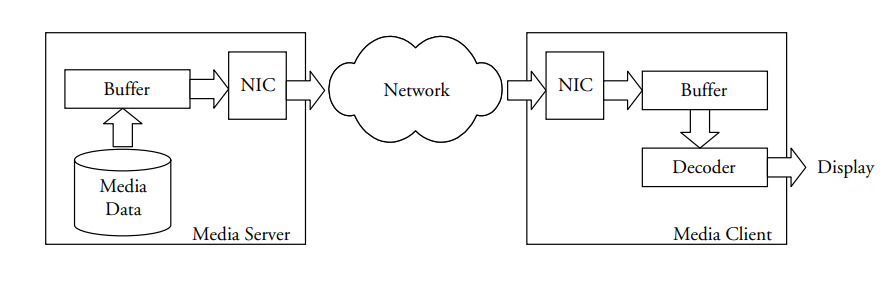
\includegraphics[width=1\linewidth]{Capturar.PNG}
	\caption[Representação de um arquitetura de tempo real genérica]{Arquitetura genérica de transmissão em tempo real}
	\label{fig:graficosVariandoTamanhoRede}
\end{figure}

\section{Sistema distribuído aberto}

Esta arquitetura é a que levarei em consideração na implementação do projeto. O
servidor que será implementado utilizando um microcomputador contem a câmera e
sistema operacional para realizar o processamento e transmissão dos dados de
multimídia. Outra alternativa seria o microcomputador apenas enviar os fluxo de
vídeo para um terceiro servidor que faria o processamento da imagem caso a
capacidade daquele não seja suficiente, resultando em um sistema distribuído.
Essa outra abordagem também respeita a arquitetura citada acima.

\section{Framework de desenvolvimento front end}

Como é de se esperar, um sistema que permite a visualização em tempo real
necessitará de um meio para apresentar ao usuário as saídas e o resultado do
processamento delas. Como se trata de um sistema de segurança, o mais viavel é
que o usuário sempre tenha em mãos o dispositivo que fornece a imagem, ou seja,
o \emph{smartphone}. Portanto, faz sentido utilizar um \emph{framework} que
permita a criação de um front end mobile. Além disso, a aplicação resultante
deverá ser replicável em múltiplos dispositivos, para que o usuário não seja
tolhido por não ter o meio adequado. Dadas essas condições, o \emph{framework}
que satisfaz elas é o \emph{React Native}

O React Native é um framework de desenvolvimento mobile híbrido (iOS e Android
simultâneamente) voltado para a construção de interfaces de usuário criado pelo
facebook, utilizando \emph{javascript} com a linguagem de programação e
compilando-o de forma que seja executável pela plataforma nativa. Vale lembrar
que o React Native não é uma solução \emph{full-stack} que vai lidar com tudo
desde o banco de dados à atualizações em tempo real de \emph{web sockets}. Ele
é simplesmente a \emph{View layer} da aplicação. \cite{boduch2017react}

\section{Tecnologias de desenvolvimento back end}

O back end é a parte do sistema que realizará o processamento da imagem que
consiste de um servidor contendo o banco de dados e uma aplicação que fornece
os \emph{endpoints} responsáveis pela comunicação com o front end. Nesses
\emph{endpoints}, o usuário consegue fazer o envio, requisição e alteração de
dados por meio da abstração fornecida pelo front end.

% Neste trabalho, o back end é responsável pelo processamento da imagem assim como pela criação do 
% canal de transmissão em tempo real dela. Além disso, existirá um \emph{endpoint} que permite
% o cadastro de um rosto específico, evitando que o sistema emita um alerta para essa pessoa.

Neste trabalho, a aplicação do \emph{back end} será feita utilizando o
\emph{NodeJS}, que é um ambiente de execução de javascript no servidor baseado
em \emph{event-driven architecture} capaz de entrada e saída assíncrona, muito
utilizado em aplicações de comunicação em tempo real. \cite{aboutnodejs} Além
disso, Em Node.js, HTTP é um cidadão de primeira classe, projetado para que
tenha um alta taxa de fluxo e baixa latência. Isso torna o Node.js uma ótima
escolha para servir como base para uma biblioteca web ou para um framework.
\cite{NodeJSaboutoriginal}. Mais um motivo para a utilização de Node.js, é a
grande quantidade de módulos disponíveis no npm. Este projeto particularmente
utilizará vários deles, sendo os principais o Express e o node-media-server. O
primeiro facilita a criação da aplicação web no servidor, e o segundo servirá
para utilizar o protocolo RTMP, que é o ideal para transmissão de vídeo e áudio
em alta performance.

Também é necessária a implementação de um banco de dados que se comunicará com
a aplicação do servidor. Para este projeto, foi escolhido o PostgreSQL, sendo
ele um banco de dados relacional de código aberto. Este sistema de banco de
dados foi escolhido por possuir \emph{Write-ahead Logging},
\emph{point-in-time-recovery}. Essas duas características são importantes para
garantir a confiabilidade e a possível recuperação dos dados em caso de perda.
Além disso, a comunidade ativa do PostgreSQL é responsável por criar diversas
extensões e alguma delas podem ajudar no desenvolvimento do projeto. O último
aspecto importante dessa escolha, é que esse sistema de banco de dados também
permite \emph{multi-factor authentication}. \cite{aboutPostgre}

Uma última camada de segurança da aplicação é necessária, de forma que tanto as
informações do usuário quanto o servidor em si estejam protegidos de possíveis
ataques. Para proteger o servidor de acesso indevido aos \emph{endpoints} vou
utilizar o JSON Web Token (JWT). O JSON Web Token é um meio de representar
reivindicações à serem transferidas entre duas partes. Os dados são codificados
com um JSON que é usado como o \emph{payload} de uma estrutura JSON Web
Encryption (JWE), permitindo que essas reivindicações sejam assinadas
digitalmente ou a integridade protegida com \emph{Message Authentication Code}
ou criptografada. \cite{jsonwebtoken}

\section{Algoritmo de reconhecimento facial}

 (Separe isso em openCV e Haar Cascade.)

Para a funcionalidade de reconhecimento facial da câmera, usarei uma biblioteca
de código aberto de \emph{computer vision} chamada \emph{OpenCV}. Essa
biblioteca possui mais de 2500 algoritmos otimizados, incluindo os clássicos e
os mais recentes do estado da arte. Eles podem ser utilizados para detectar e
reconhecer faces, identificar objetos classificar ações humanas em vídeo e
mais. \cite{opencv}. Ela suporta múltiplas linguagens incluindo Java, C++ e
Python. para este trabalho, será usada a biblioteca em Python.

Para realizar o reconhecimento facial, é preciso conseguir antes reconhecer que
há um rosto em vídeo. O método que utilizarei, facilitado pelo \emph{OpenCV}, é
o chamado \emph{Haar Cascades} \cite{viola2001rapid}. Este algoritmo é baseado
em \emph{machine learning} onde a função de cascata é treinada por meio de
muitas imagens positivas e negativas. No caso, as imagens positivas são várias
fotos com rostos e as negativas são fotos sem rosto. O conceito de
classificadores em cascata desse algoritmo por sua vez, vem do fato de que no
lugar de aplicar as características encontradas numa única etapa, elas são
agrupadas em diferentes estágios de classificação uma a uma. Se um desses
estágios falhar, então a imagem é descartada, desconsiderando as
características remanescentes nela. Assim sendo, a foto que passar por todos os
estágios é uma região de um rosto.

A próxima parte do processo envolve usar o algoritmo que reconhece que existe
um rosto no vídeo junto com um outro algoritmo que reconhecerá à quem pertence
este rosto. Para o algoritmo classificador reconhecedor que será usado agora,
são necessárias varias imagens do rosto a ser reconhecido, que serão
convertidas para \emph{grayscale}, dessa forma mantendo o plano de luminância e
separando o de crominância de cada imagem o que por sua vez reduz a quantidade
de informação desnecessária presente e, por isso, facilita a identificação das
características importantes para classificação. Em seguida, será usado o
algoritmo Local Binary Patterns Histogram (LBPH) para realizar o treinamento do
modelo que reconhecerá os rostos usando as imagens preparadas anteriormente. O
LBPH foi escolhido por funcionar bem com as imagens em \emph{grayscale} e ser
capaz de desconsiderar a luminosidade como característica importante, como
mostra a figura abaixo:

\begin{figure}[!ht]
	\centering
	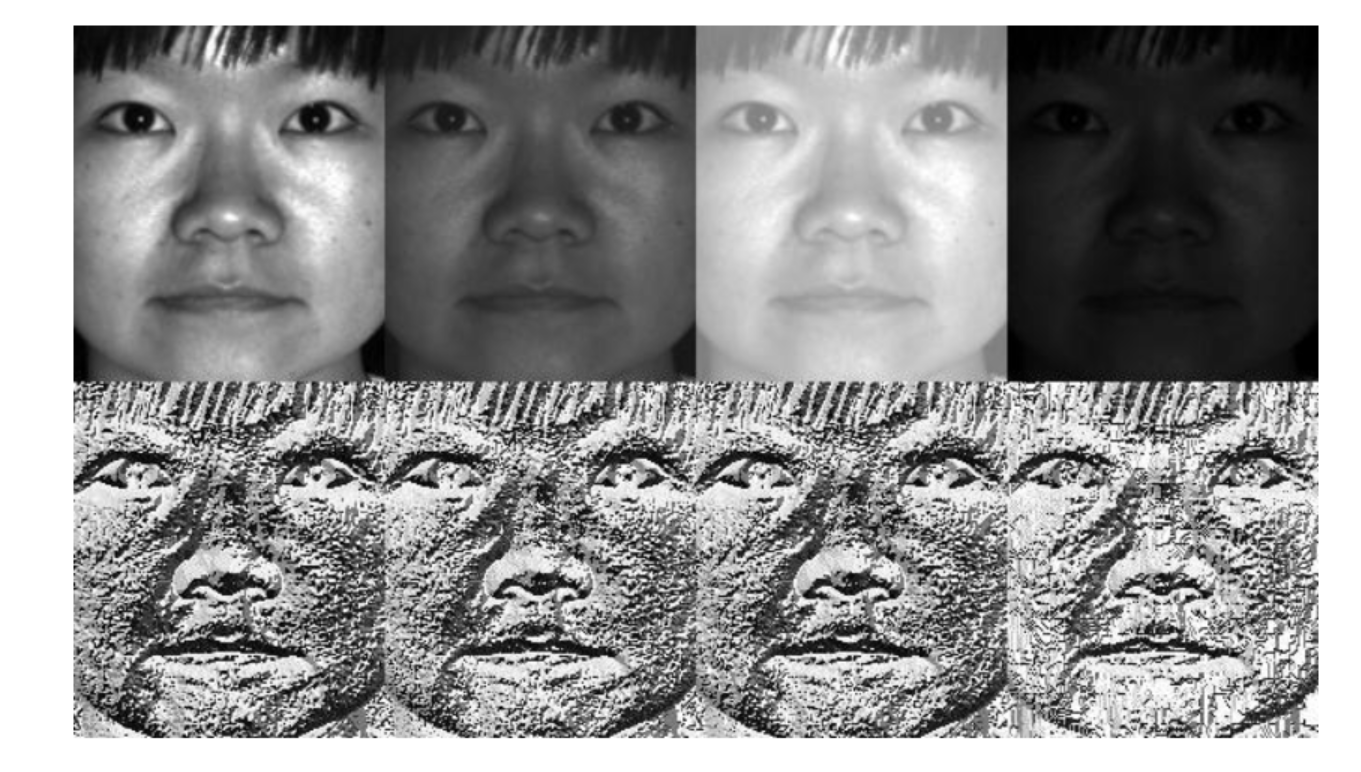
\includegraphics[width=0.7\linewidth]{grayscale.PNG}
	\caption[De \emph{grayscale} para LBP
	]{Imagens resultantes do algoritmo LBP abaixo, geradas à partir da imagem em \emph{grayscale} acima.}
	\label{fig:graficosVariandoTamanhoRede}
\end{figure}
% é o proposto por Paul Viola e Michael Jones no 
% artigo  "Rapid Object Detection using a Boosted Cascade of Simple Features" em 2001. É uma abordagem
% baseada em Machine Learning em que uma função \emph{cascade} é treinada com o uso de muitas imagens
% positivas e negativas.

\section{Arquitetura de microsserviços}

Explicar aqui o que são microsseviços e como eles funcionam. Fazer talvez uma
comparação em relação à uma monolito

\section{Arquitetura Monolítica}

Explicar aqui como funciona uma arquitetura monolítica e quais as desvantagens
e vantagens em relação ao microsserviço.

\section{Protoclo RTSP}

Explciar como o protocolo RTSP é usado para pegar o feed das imagens. Existe o
RFC to protocolo RTSP aqui:
% https://www.rfc-editor.org/rfc/rfc2326#page-71

\section{Conteinerização}

Explicar aqui o porquê de servir o software no docker

\section{Diagrama de Componentes}

O diagrama de componentes é uma ferramenta da UML (Unified Modeling Language).
Ele tem como objetivo visualizar a organização e as relações entre diferentes
componentes em um sistema de software. Enquanto outros diagramas focam na
funcionalidade do sistema, o diagrama de componentes se concentra no aspecto
estrutural.

Um diagrama de componentes representa partes modulares de um sistema, chamadas
de componentes. Estes componentes podem ser físicos (como bibliotecas, módulos,
arquivos) ou conceituais e estão conectados através de interfaces. Estas
interfaces são os pontos de interação entre os componentes.

Características dos diagramas de componentes:
\begin{itemize}
	\item Mostram as dependências entre os componentes.
	\item Identificam as interfaces que conectam os componentes.
	\item Auxiliam na modularização e reutilização de software.
	\item Oferecem uma visão da arquitetura do sistema.
\end{itemize}

Ao trabalhar com diagramas de componentes, as equipes podem compreender melhor
a estrutura do sistema e identificar áreas para atenção ou desenvolvimento.

Abaixo, um exemplo de um componente e suas partes:

\begin{figure}[!ht]
	\centering
	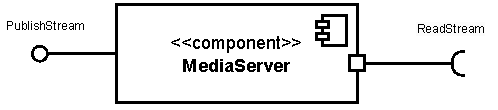
\includegraphics[width=0.8\linewidth]{example_diagram.pdf}
	\caption[Componente de exemplo]{Componente, provendo uma interface e com requerimento de outra}
	\label{fig:graficosVariandoTamanhoRede}
\end{figure}

O componente é representado pela estrutura retangular. O ícone no topo direito
do retângulo é opcional, sendo uma especificação do UML 1.4. Na Figura, a
bolinha à esquerda com a legenda PublishStream indica uma interface provida, e
o semi círculo indica uma interface requerida.

Uma interface fornecida é aquela que é realizada diretamente pelo próprio
componente, ou realizada por um dos classificadores que implementam o
componente, ou ainda fornecida por uma porta pública do componente. Na notação
de pirulito, temos a interface fornecida do componente. No exemplo, o
componente de MediaServer fornece (implementa) a interface de PublishStream.

Uma interface necessária é aquela designada por uma dependência de uso do
próprio componente, ou designada por uma dependência de uso de um dos
classificadores que implementam o componente, ou ainda é exigida por uma porta
pública do componente. No exemplo, o componente MediaServer requer a interface
ReadStream.

\section{Versionamento Semântico (SEMVER)}

O \textit{SEMVER}, abreviação de Versionamento Semântico, é uma convenção de
nomenclatura usada para gerenciar e comunicar eficazmente as mudanças em
versões de software. Ele cria uma maneira
compreensível de representar as mudanças em software através do número de sua
versão.

A estrutura básica de um número de versão SEMVER é \textit{MAJOR.MINOR.PATCH},
onde:

\begin{itemize}
	\item \textit{MAJOR} é incrementado para mudanças incompatíveis que requerem que o usuário faça algo diferente.
	\item \textit{MINOR} é incrementado quando são feitas adições em um modo compatível, ou seja, quando funcionalidades são adicionadas sem alterar o comportamento das funcionalidades existentes.
	\item \textit{PATCH} é incrementado após correções de bugs que são compatíveis e não afetam o funcionamento global do software de maneira significativa.
\end{itemize}

Além destes três números principais, o SEMVER também permite a adição de
etiquetas pré-lançamento e de build, que podem ser usadas para representar
versões alfa, beta, candidatas a lançamento, entre outros.

O principal benefício de adotar o \textit{SEMVER} é a clareza. Ao olhar para o
número de versão de um software, os desenvolvedores podem rapidamente entender
a natureza e a magnitude das mudanças, facilitando decisões sobre a atualização
ou integração de dependências.  \cite{semver}

\section{Daemon}

Explicar o conceito de Daemon e o porquê de ser últil manter o software rodando
como um processo segundo plano

\section{Liskov Substitution Principle}

Falar um pouco aqui sobre o princípio de Liskov e como ele é usado por exemplo
no recorder.

\section{Proxy}

Explicar o porquê de às vezes usar um proxy. Às vezes queremos dar um feed de
imagem, mas não tem como fazer uma conexão direta ao sistema que está provendo
diretamente a imagem com RTSP. Tanto porque o sistema não consegue lidar com
muitas requisições ao mesmo tempo, ou porque ele está numa intranet que precisa
de um acesso seguro para prover ao resto da rede.

\section{Licenças de Software}

Explciar o porquê de usar uma licença de software adequada. E como diferentes
Licenças de Software podem afetar como esse sistema é construído e mantido.
Citar aquela licença (Acho que é a BPD) que pode absolutamente obliterar todo
mundo que já estava usando um software específico.

\section{Encodings de vídeo e som}

Tenho que citar alguns encodings usados.

\subsection{H.264}

O que acontece nesse tipo de encoding? Em quais cenários ele é usado? Quais os
problemas dele?

Essa informação aqui é importante para o streaming com WebRTC

WebRTC doesn't support H264 streams with B-frames: H264 is a video compression
codec. In H264 encoding, three types of frames are used: I-frames (Intra
frames), P-frames (Predictive frames), and B-frames (Bidirectional predictive
frames). The error message is stating that WebRTC does not support H264 streams
that include B-frames.

B-frames depend on both previous and future frames to derive their data, and
this can cause issues in real-time streaming scenarios like those handled by
WebRTC, where latency and real-time performance are crucial. Therefore, WebRTC
doesn't support H264 streams with B-frames.

\section{Tecnologia de Hardware}

Todos os algoritmos que irão processar a imagem da câmera e aplicação do back
end precisam ficar alocados num servidor. Assim sendo, foi escolhido um
raspberry pi zero W 1.1 para ser usado como o dispositivo que funcionará como
servidor. Além disso, o Camera Module V2 será responsável por captar a imagem.
Se fizermos uma comparação com os dispositivos de monitoramento presentes no
mercado, esses dispositivos não são muito potentes. A empresa força tarefa de
Uberlândia que fornece serviços de segurança e portaria remota, por exemplo,
utiliza câmeras IP da Intelbras, muitas delas com sensores de visibilidade
noturna, como o modelo VIP 3230 B SL. Por meio de uma conexão de rede, a
informação de vídeo dessas câmeras vai para os servidores da empresa que
possuem alta capacidade de processamento. Entretanto, mesmo com a capacidade
reduzida dos dispositivos que serão usados neste trabalho, os algoritmos de
reconhecimento facial, a aplicação do servidor e o front end poderão ser
transferidos para outros melhores.

% raspberry pi zero W V 1.1

\chapter{Método de Desenvolvimento}

A metodologia selecionada para o avanço deste projeto se baseia, inicialmente,
em um exame das soluções de software atualmente presentes no mercado. O
objetivo é compreender suas características, funcionalidades e deficiências.
Esse estudo, de caráter essencialmente qualitativo, procura identificar
tendências, padrões e lacunas nas soluções existentes.

Em seguida, serão exploradas as tecnologias e técnicas comumente adotadas na
indústria. Essa investigação abrange desde protocolos de transporte até
algoritmos sofisticados de compressão e reconhecimento, assim como casos de
vulnerabilidades de segurança. O intuito é discernir os padrões de uso e as
preferências do setor.

Dentro desse contexto, uma análise focada no SSCS será realizada.
Investigaremos se ele propõe uma reinvenção dessas soluções padrão ou se opta
por uma integração harmônica com elas. Esta etapa é crucial para entender a
proposta de valor e o diferencial que o sistema proposto oferece em relação às
alternativas tradicionais.

Posteriormente, adentraremos na esfera econômica, conduzindo uma pesquisa sobre
os custos envolvidos. Essa avaliação não se restringirá apenas aos valores de
aquisição de software ou hardware, mas também contemplará os gastos
operacionais, incluindo a execução de softwares e os custos de aquisição,
manutenção e atualização de hardwares.

\section{Estado da Arte de Câmeras de Vigilância}

Diversas soluções de vigilância estão atualmente disponíveis no mercado, cada
uma adotando um conjunto único de padrões e tecnologias. Entre as várias
opções, as câmeras CCTV (\textit{\foreignlanguage{english}{Closed-circuit
		television}}) emergem como um sistema tradicional e amplamente empregado.
Curiosamente, o conceito de CCTV remonta a 1927, quando o físico russo Léon
Theremin desenvolveu o primeiro dispositivo desse tipo, dando origem à primeira
geração de sistemas de vigilância \cite{glinsky2000theremin}. Esse sistema
consiste em um número de câmeras localizadas em múltiplas posições remotas e
conectadas a um conjunto de monitores, geralmente em uma única sala de
controle, através de switches (uma matriz de vídeo). Ao contrário de soluções
mais modernas que utilizam transmissão via IP, as câmeras CCTV são
frequentemente associadas a sistemas de transmissão analógica, embora modelos
mais recentes possam incorporar capacidades digitais e transmissão pela web.
Atualmente, os modelos mais comuns de câmeras de vigilância para uso comercial
já possuem integração direta à internet usando o protocolo IP.

O avanço tecnológico nas câmeras de vigilância levou ao desenvolvimento de
sistemas semi-automáticos, conhecidos como sistemas de vigilância de segunda
geração. A maior parte da pesquisa nesses sistemas é baseada na criação de
algoritmos para detecção automática em tempo real de eventos, auxiliando o
usuário a reconhecer os eventos.

Seguindo essa mesma tendência tecnológica, chegamos então à terceira geração,
que se refere aos sistemas de vigilância concebidos para lidar com um grande
número de câmeras, uma dispersão geográfica de recursos, muitos pontos de
monitoramento, e para espelhar a natureza hierárquica e distribuída do processo
humano de vigilância. Os principais objetivos que se espera de uma aplicação
genérica de vigilância visual de terceira geração, baseada nas exigências do
usuário final, são fornecer uma boa compreensão da cena, orientada para atrair
a atenção do operador humano em tempo real, possivelmente em um ambiente
multi-sensorial, informações de vigilância e usando componentes padrões de
baixo custo.

\section{Tecnologias e técnicas comuns}

\subsection{métodos de transmissão}

No quesito dos métodos de transmissão multimídia por essas câmeras, temos três
métodos principais: \textit{\foreignlanguage{english}{streaming}} tradicional,
\textit{\foreignlanguage{english}{download}} progressivo, e
\textit{\foreignlanguage{english}{streaming}} adaptativo. Cada um deles tem
suas vantagens e desvantagens quanto aos critérios de latência, qualidade,
requerimentos de processamento e compatibilidade com outros tipos de software.
O \textit{\foreignlanguage{english}{Streaming}} tradicional requer um protocolo
\textit{\foreignlanguage{english}{stateful}} que estabelece uma sessão entre o
servidor e o cliente. Nesse último método, a mídia é transmitida como uma
corrente constante de pacotes por UDP ou TCP.
% Como exemplo o Real Time
% Streaming Protocol (RTSP) , baseado no Real-time Transport Protocol (RTP), que
% é o mais comum para a transmissão de vídeo nas câmeras por IP: a vasta maioria
% delas o integram como padrão.
Já no método do streaming por \textit{\foreignlanguage{english}{download}}
progressivo, usa-se um servidor HTTP para transferir o vídeo entre o cliente e
o servidor, de maneira \textit{\foreignlanguage{english}{stateless}}. Os
clientes fazem requisições de multimídia, que é enviado progressivamente para
um buffer local. Assim que ele tem informação o suficiente, o vídeo começa a
tocar. Se a taxa de \textit{\foreignlanguage{english}{playback}} excede a taxa
de transmissão de dados, então o vídeo é interrompido até que o buffer seja
preenchido adequadamente. O \textit{\foreignlanguage{english}{streaming}}
adaptativo por sua vez, consiste em detectar a largura de banda de rede e
capacidade de CPU do cliente para ajustar a qualidade do vídeo transmitido
buscando a melhor opção para as condições dadas. Isso requer um
\textit{\foreignlanguage{english}{encoder}} para prover vídeo em múltiplos
\textit{\foreignlanguage{english}{bit rates}} diferentes, ou múltiplos
\textit{\foreignlanguage{english}{encoders}} e pode ser usada uma Content
Delivery Network (CDN) para aumentar a escalabilidade. É comum em streaming
adaptativo utilizar a técnica de \textit{\foreignlanguage{english}{stream
		switching}}. Esse é um método híbrido que usa HTTP como o protocolo de entrega
no lugar de definir um novo protocolo. Os dados de multimídia são segmentados
em pequenas partes de mesmo tamanho, codificados no formato desejado e
armazenadas em um servidor. Os clientes então requisitam os segmentos
sequencialmente por download progressivo e eles são tocados em ordem já que são
contíguos. O resultado é uma experiência de usuário praticamente livre de
gargalos de buffering em condições normais de rede e CPU.

\subsection{algoritmos de reconhecimento de imagem}

Existem duas abordagens convencionais principais para detecção de objetos:
"diferença temporal" e "subtração de fundo". A primeira abordagem consiste na
subtração de dois quadros consecutivos seguida por uma limiarização. A segunda
técnica é baseada na subtração de um modelo de fundo ou referência e a imagem
atual seguida por um processo de rotulagem. Além destas, existem abordagens
baseadas em aprendizado de máquina, como o Haar Cascade, onde classificadores
são treinados usando imagens positivas (com objetos) e imagens negativas (sem
objetos) para criar uma função que pode ser usada para detectar algo específico
em outras imagens. O Haar Cascade é especialmente eficaz para detecção de faces
e oferece processamento rápido, sendo uma opção viável para detecção em tempo
real. No entanto, pode apresentar desafios em cenas complexas ou com objetos
ocluídos. Além disso, há técnicas mais avançadas como Deep Learning, que,
através de Redes Neurais Convolucionais (CNNs) e variações como R-CNN, Faster
R-CNN, YOLO, e SSD, conseguem alta precisão e robustez na detecção de diversos
tipos de objetos em cenários variados, embora exijam um grande volume de dados
para treinamento e recursos computacionais consideráveis. Diferentemente das
técnicas de subtração de fundo e diferença temporal, que são menos intensivas
computacionalmente, as técnicas de aprendizado de máquina e aprendizado
profundo podem requerer mais recursos e um conjunto de treinamento de dados,
mas oferecem maior precisão e capacidade de generalização, tornando-se
preferíveis em aplicações mais complexas ou quando a alta precisão é crucial.

\subsection{armazenamento e compressão}

\subsection{vulnerabilidades de segurança}

No quesito dos riscos de segurança, as câmeras IP apresentam várias
vulnerabilidades que podem expô-las a ameaças. Uma das falhas mais comuns é a
utilização de credenciais de login padrão, que são facilmente acessíveis para
qualquer pessoa com conhecimento básico em segurança de rede. Além disso,
políticas de autenticação fracas frequentemente permitem a seleção de senhas
simples e fáceis de adivinhar. A criptografia inadequada de informações
confidenciais é outro ponto de preocupação, pois muitas vezes os dados são
transmitidos sem qualquer processo de criptografia, tornando-os suscetíveis a
interceptações e ataques. Como exemplo dessas falhas, em \cite{9116392} uma
câmera smart identifica como Onvif YY HD passou por um teste de penetração.
Nesse teste, um ataque do tipo man in the middle (MITM) foi capaz de visualizar
em texto plano todos os dados transmitidos pela câmera, inclusive credenciais.

% TODO: verificar se essa parte toda aqui que eu falei sobre os protocolos faz sentido de estar aqui.
% ao meu ver perdeu um pouco do sentido e parece mais fazer parte do desenvolvimento em si

% Usar esse link como referência pode ser bom:
% https://stackoverflow.com/questions/35697778/what-streaming-protocols-can-publish-video-audio?rq=2

% E esse aqui tem um report visual ! com informações de quais protocolos estão sendo usados:

% https://www.wowza.com/blog/hls-vs-webrtc#delivery-method

\chapter{Revisão Bibliográfica}
%TCC:
Um ou mais capítulos (por exemplo, se há duas linhas de trabalhos
relacionados).

\chapter{Desenvolvimento}
Inicialmente, é vantajoso estabelecer um meio de simular um fluxo de vídeo para
o SSCS processar. Esta abordagem facilita os testes e proporciona um ambiente
de desenvolvimento que replica com fidelidade as condições sob as quais o
sistema operará quando implementado em um ambiente de produção. É importante
esclarecer que, ao referir-se a "sistema em produção", estamos discutindo a
aplicação prática do software em ambientes comerciais, residenciais, ou outros
contextos reais onde a vigilância é empregada para segurança e monitoramento.

No desenvolvimento do sistema, foi empregado o MediaMTX \cite{mediamtx}, um
servidor de mídia em tempo real de código aberto que facilita a publicação,
leitura, gravação e roteamento de streams de vídeo. Este software foi
originalmente concebido para funcionar como um roteador de mídia de ponta a
ponta, proporcionando uma plataforma robusta a partir da qual o SSCS pode
acessar e consumir streams de vídeo. Entretanto, para que o servidor seja
operacional, é necessário que a mídia seja publicada nele. Conforme indicado na
documentação do MediaMTX, uma das abordagens recomendadas para isso é a
utilização do ffmpeg, um framework de multimídia que permite a codificação,
decodificação, transcodificação, muxing, demuxing, streaming e reprodução de
dados de mídia. Através do ffmpeg \cite{ffmpeg}, é possível enviar streams de
vídeo para o servidor MediaMTX, criando assim um ambiente propício para a
integração e operação eficiente com o SSCS.

Como é muito comum que sistemas de vigilância possuam várias câmeras ao mesmo
tempo, faz sentido a arquitetura abaixo, que lida exclusivamente com a parte da
transmissão para o servidor de mídia SSCS.

\begin{figure}[!ht]
	\centering
	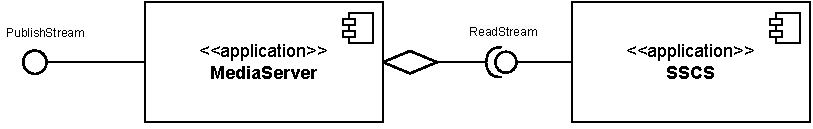
\includegraphics[width=0.8\linewidth]{arch1.pdf}
	\caption[Exemplo de arquiteutra de transmissão]{Arquitetura de transmissão, múltiplas fontes para um servidor de mídia}
	\label{fig:graficosVariandoTamanhoRede}
\end{figure}

% \begin{figure}[!ht]
% 	\centering
% 	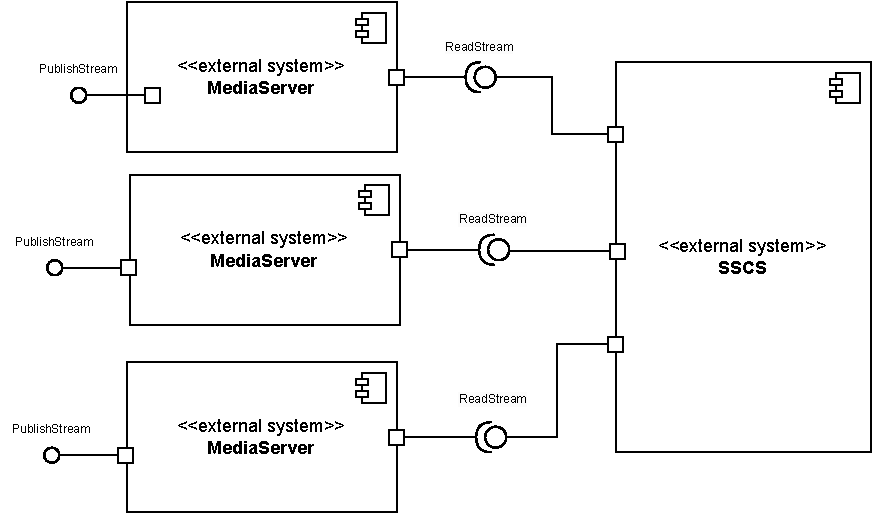
\includegraphics[width=0.8\linewidth]{arch2.pdf}
% 	\caption[Exemplo de arquiteutra de transmissão]{Arquitetura de transmissão, múltiplos servidores de mídia}
% 	\label{fig:graficosVariandoTamanhoRede}
% \end{figure}

A ilustração representa um cenário onde câmeras ou outras fontes de streaming
multimídia podem transmitir streams para um servidor intermediário. O servidor
de mídia intermediário provê uma interface PublishStream que permite o
recebimento de streams de multimídia por várias fontes diferentes. O losango
indica que o MediaServer é um agregador, o que significa que ele pode interagir
com múltiplas aplicações do SSCS ao mesmo tempo. Porém, trata-se de uma
associação fraca: o MediaServer pode funcionar sozinho sem o SSCS.

Os servidores intermediários desempenham o papel de proxies para o servidor que
opera o SSCS. A utilização de um servidor de mídia como proxy apresenta
diversas vantagens. Por exemplo, pode ser necessário converter o protocolo de
transmissão de RTSP para WebRTC ou HLS, realizar balanceamento de carga, ou até
mesmo implementar autenticação externa.

%TCC:
%TCC:
%TCC:
%TCC:

% ---
% Conclusão
% ---
\chapter[Conclusão]{Conclusão}
%TCC:
E daí?

% ----------------------------------------------------------
% ELEMENTOS PÓS-TEXTUAIS
% ----------------------------------------------------------
\postextual

% ----------------------------------------------------------
% Referências bibliográficas
% ----------------------------------------------------------
\bibliography{abntex2-modelo-references}

%% ----------------------------------------------------------
%% Apêndices TCC: só mantenha se for pertinente.
%% ----------------------------------------------------------

% ---
% Inicia os apêndices
% ---
\begin{apendicesenv}

	% Imprime uma página indicando o início dos apêndices
	\partapendices

	% ----------------------------------------------------------
	\chapter{Quisque libero justo}
	% ----------------------------------------------------------

	\lipsum[50]

	% ----------------------------------------------------------
	\chapter{Coisas que fiz e que achei interessante mas não tanto para entrar no corpo do texto}
	% ----------------------------------------------------------
	\lipsum[55-57]

\end{apendicesenv}
% ---

% ----------------------------------------------------------
% Anexos %TCC: so mantenha se pertinente.
% ----------------------------------------------------------

% ---
% Inicia os anexos
% ---
\begin{anexosenv}

	% Imprime uma página indicando o início dos anexos
	\partanexos

	% ---
	\chapter{Eu sempre quis aprender latim}
	% ---
	\lipsum[30]

	% ---
	\chapter{Coisas que eu não fiz mas que achei interessante o suficiente para colocar aqui}
	% ---

	\lipsum[31]

	% ---
	\chapter{Fusce facilisis lacinia dui}
	% ---

	\lipsum[32]

\end{anexosenv}

%---------------------------------------------------------------------
% INDICE REMISSIVO
%---------------------------------------------------------------------

\printindex

\end{document}